\section{Fundamental groupoid revisited}

Recall the adjunction 
    \begin{tikzcd}
         \Set_{\Delta}
        \arrow[r, shift left, "\tau"]
        &
        \Gpd
        \arrow[l, shift left, "N"]
    \end{tikzcd}
and suppose that $X \in \Set_{\Delta}$ is a Kan complex.

\begin{construction}

The homotopy category of $X$ is called $\H0(X)$ is defined as follows:
\begin{itemize}
    \item 
    $\Ob(\H0(X))=X_0$
    \item 
    $\hom_{\H0(X)}(X,Y) = \{f \in X_1 \mid d_1(f)=X , d_0(f)=y \} / \sim$
\end{itemize}

Recall that a $2$-simplex of $X$
\[
\begin{tikzcd}
    &
    Y
    \arrow[rd,"g"]
    &\\
    X
    \arrow[ru, "f"]
    \arrow[rr,"h"']
    &
    &
    Z
\end{tikzcd} 
\]
should be a "witness" of the fact the $h$ is a composition of $f$ and $g$.
\end{construction}

\begin{problem}
    Why are there different choices of relation $\sim$?
    Given as follows
    \[
    \begin{tikzcd}
        &
        X
        \arrow[rd,"f"]
        &\\
        X
        \arrow[ru, "1_X"]
        \arrow[rr,"g"']
        &
        &
        Y
    \end{tikzcd} 
    = f \sim_1 g
    \qquad
    \begin{tikzcd}
        &
        Y
        \arrow[rd,"1_Y"]
        &\\
        X
        \arrow[ru, "f"]
        \arrow[rr,"g"']
        &
        &
        Y
    \end{tikzcd} 
    = f \sim_2 g
    \]
    \[
    \begin{tikzcd}
        &
        X
        \arrow[rd,"g"]
        &\\
        X
        \arrow[ru, "1_X"]
        \arrow[rr,"f"']
        &
        &
        Y
    \end{tikzcd} 
    = f \sim_3 g
    \qquad
    \begin{tikzcd}
        &
        Y
        \arrow[rd,"1_Y"]
        &\\
        X
        \arrow[ru, "g"]
        \arrow[rr,"f"']
        &
        &
        Y
    \end{tikzcd} 
    = f \sim_4 g
    \]
    where $1_X\coloneqq s_0(X)$. 
    What remains to be shown is that all these are equivalence relations and are in fact the same.
\end{problem}

Lecture 26.11

\begin{prop}
    The four relations above are the same and are equivalence relations.
\end{prop}

\begin{proof}
    We show $(f \sim_3 g \implies f \sim_1 g)$, thus let 
    \[
    \begin{tikzcd}
        &
        X
        \arrow[rd,"g"]
        &\\
        X
        \arrow[ru, "1_X"]
        \arrow[rr,"f"']
        &
        &
        Y
    \end{tikzcd} 
    = \sigma \in X_2
    \]
    We can glue the following $2$-simplices 
    \[
    \begin{tikzcd}
        &
        X
        \arrow[rd,"1_X"]
        &\\
        X
        \arrow[ru, "1_X"]
        \arrow[rr,"1_X"']
        &
        &
        X
    \end{tikzcd} 
    =c^2(X)
    \qquad
    \begin{tikzcd}
        X
        \arrow[rr,"1_X"]
        \arrow[rd,"g"']
        &
        &
        X
        \arrow[ld, "g"]
        \\
        &
        Y
        &
    \end{tikzcd}
    =s_0(g)
    \]
    \[
    \begin{tikzcd}
        X
        \arrow[dd,"f"']
        \arrow[rd,"1_X"]
        &
        \\
        &
        X
        \arrow[ld,"g"]
        \\
        Y
    \end{tikzcd}
    =\sigma
    \]
    to obtain a $3$-horn
    \[
    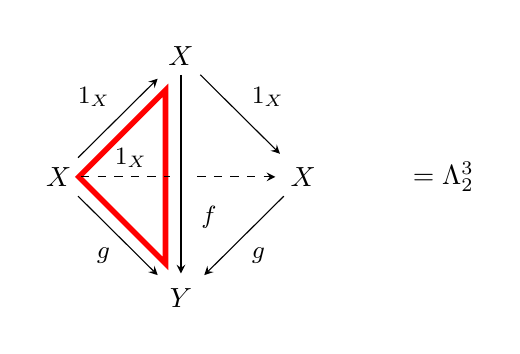
\begin{tikzpicture}[>=stealth,->,shorten >=2pt,looseness=.5,auto]
            \matrix[anchor=center, column sep=1cm, row sep=1cm] at (0,0)
            {
                                & \node(X_1) {$X$};   &                 &\\
             \node(X_0) {$X$};     &                  & \node(X_2) {$X$};& \node(X_24) {$=\Lambda_2^3$};  \\
                                & \node(X_3) {$Y$};   &                 &\\
            };
            \draw[line width=2pt,color=red] (-1.2,1.1) -- (-1.2,-1.1) -- (-2.3, 0) -- cycle;
            \begin{scope}[every node/.style={font=\small\itshape}]
                \draw (X_1) -- node [midway] {$1_X$} (X_2);
                \draw (X_0) -- node [midway] {$1_X$} (X_1);
                \draw (X_0) -- node [midway, swap] {$g$}(X_3);
                \draw [dashed] (X_0) -- node [near start] {$1_X$}(X_2);
                \draw [-,line width=8pt,draw=white]
                (X_1) -- node [pos=0.7] {$f$} (X_3);
                \draw (X_1) -- (X_3);
                \draw (X_2) -- node [midway] {$g$} (X_3);
            \end{scope}
    \end{tikzpicture} 
    \]
    The red $2$-simplex is exactly the one of the equivalence relation $f \sim_1 g$. 
    Since $X$ is an inner Kan complex by assumption, we have the desired horn extension.
    The other direction were part of an exercise and will be included here eventually.
    What remains to be shown, is that it is an equivalence relation.
    \begin{itemize}
        \item 
        (Reflexivity) 
        Let $X \xrightarrow{f} Y$ be in $X_1$, then we have the 2-simplex
        \[
        \begin{tikzcd}
            &
            X
            \arrow[rd,"f"]
            &\\
            X
            \arrow[ru, "1_X"]
            \arrow[rr,"f"']
            &
            &
            Y
        \end{tikzcd} 
        \]
        which means that $\sim$ is associative.
        \item 
        (Symmetry)
        We have the following chain of equivalences
        \[
        f\sim g \iff f\sim_1 g \iff f \sim_3 g \iff g \sim_1f \iff g \sim f
        \]
        \item 
        (Transitivity)
        Let $f\sim g$ and $g \sim h$.
        Consider the following diagrams
        \[
        \begin{tikzcd}
            &
            X
            \arrow[rd, "f"]
            &
            \\
            X
            \arrow[rr, "g"]
            \arrow[ru, "1_X"]
            \arrow[rd, "h"']
            &
            &
            Y
            \arrow[ld,"1_Y"]
            \\
            &
            Y
            &
        \end{tikzcd}
        \qquad
        \begin{tikzcd}
            X
            \arrow[dd, "f"']
            \arrow[rd, "f"]
            \\
            &
            Y
            \arrow[ld, "1_Y"]
            \\
            Y
        \end{tikzcd}
        \] which glued at $1_Y$ and $f$ result in the following horn
        \[
        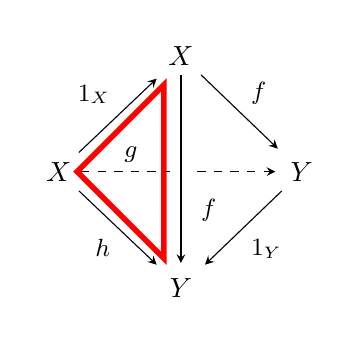
\begin{tikzpicture}[>=stealth,->,shorten >=2pt,looseness=.5,auto]
            \matrix[anchor=center, column sep=1cm, row sep=1cm] at (0,0)
            {
                                & \node(X_1) {$X$};   &                 \\
             \node(X_0) {$X$};     &                  & \node(X_2) {$Y$};  \\
                                & \node(X_3) {$Y$};   &                 \\
            };
            \draw[line width=2pt,color=red] (-0.2,1.1) -- (-0.2,-1.1) -- (-1.3, 0) -- cycle;
            \begin{scope}[every node/.style={font=\small\itshape}]
                \draw (X_1) -- node [midway] {$f$} (X_2);
                \draw (X_0) -- node [midway] {$1_X$} (X_1);
                \draw (X_0) -- node [midway, swap] {$h$}(X_3);
                \draw [dashed] (X_0) -- node [near start] {$g$}(X_2);
                \draw [-,line width=8pt,draw=white]
                (X_1) -- node [pos=0.7] {$f$} (X_3);
                \draw (X_1) -- (X_3);
                \draw (X_2) -- node [midway] {$1_Y$} (X_3);
            \end{scope}
    \end{tikzpicture}
    \]
    By the horn filling property of the inner Kan complex for a 3-horn at position 2 we get the desired $f \sim g$.
    \end{itemize}
\end{proof}

\begin{prop}
    The composition law in $\H0(X)$ is well defined, unital and associative.
\end{prop}

\begin{proof}
    Suppose that $f \sim f'$. 
    From now on we write $gf \sim h$ to mean that there exists a 2-simplex
    \[
    \begin{tikzcd}
        &
        Y
        \arrow[rd,"g"]
        &\\
        X
        \arrow[ru, "f"]
        \arrow[rr,"h"']
        &
        &
        Z
    \end{tikzcd}   
    \in X_2
    \]
    We prove that if $gf \sim h$, $gf' \sim h'$ and $gf' \sim h$ it follows that $h \sim h'$. 
    So consider the corresponding 2-simplices
    \todo{i am too lazy to do the "assemble the obvious simplex proves" right now, soooo fuck you future Vincent suuuckkaaaaa}
\end{proof}

\begin{rmk}
    \todo{what does this remark mean?}
    \begin{tikzcd}
        &&Z
    \end{tikzcd}
    $\H0 (X)$ is a well defined category when $X$ is an inner Kan complex.
\end{rmk}

\begin{prop}
    Let $X \in \SetD$ be $X$ a Kan complex, then $\H0 (X)$ is a groupoid.
\end{prop}

\begin{proof}
    Let $f \in \H0(X)$ be a morphism. 
    Consider the simplex 
    \begin{tikzcd}
        & 
        X
        \arrow[rd, "f"]
        &
        \\
        Y
        \arrow[rr, "1_Y"']
        \arrow[ru, dashed, "\exists g"]
        &&
        Y
    \end{tikzcd}
\end{proof}

\begin{cor}
    Let $X \in \SetD$ be a Kan complex, then $L \H0(X) \cong \H0(X)$.
\end{cor}

\begin{proof}
     Consider the adjunction 
     \[
     \begin{tikzcd}
        \Cat
        \arrow[r, shift left, "L"]
        &
        \Gpd 
        \arrow[l, shift left, "y'"]
    \end{tikzcd}
     \]
     Then the counit $\eta$ of the adjunction is the desired isomorphism.
     \todo{details}
\end{proof}

\begin{prop}
    Let $X \in \SetD$ be an inner Kan complex, then $H_0(X) \cong \tau X$.
\end{prop}

\begin{proof}
    Let $\mathcal{D} \in \Cat$, since $N(\mathcal{D}) \in \SetD$ is $2$-coskeletal, we have a natural bijection.
    \[
    \Hom_{\SetD}(X, N( \mathcal{D})) \isomorphism \Hom_{\SetD}(\tru_2X,\tru_2(N(\mathcal{D}))
    \]
    Consider a morphism $\tru_2(X) \xrightarrow{f} \tru_2(N(\mathcal{D}))$ given by
    \[
    \begin{tikzcd}
        \tru_2
        \arrow[d,"f"]
        &
        X\colon \dotsc 
        &
        X_2
        \arrow[r, altstackar=5]
        \arrow[d,"f_2"]
        &
        X_1
        \arrow[r,altstackar=3]
        \arrow[d,"f_1"]
        &
        X_0=\Ob(\Ho(X))
        \arrow[d,"f_0"]
        \\
        \tru_2(N(\mathcal{D}))
        &
        N(\mathcal{D})\colon \dotsc 
        &
        N(\mathcal{D})_2
        \arrow[r, altstackar=5]
        &
        N(\mathcal{D})_1
        \arrow[r,altstackar=3]
        &
        N(\mathcal{D})_0=\Ob(\mathcal{D})
    \end{tikzcd}
    \]
    Note that $N(\mathcal{D})_1=\Mor( \mathcal{D} )$.
    We have for any $\alpha \in X_1$ that $f_0(d_0(\alpha)) = \text{target} (f_1(\alpha))$ and that for any $d_1(\alpha) \xrightarrow{\alpha}d_0(\alpha)$ that $f_0(d_1(\alpha))= \text{source}(\alpha)$.
    Now for 2-simplices we have
    \[
    \alpha \sim \beta
     \begin{tikzcd}
        &
        x
        \arrow[rd,"\alpha"]
        &\\
        x
        \arrow[ru, "1_x"]
        \arrow[rr,"\beta"']
        &
        &
        y
    \end{tikzcd}   
    \xmapsto{f_2}
    \begin{tikzcd}
        &
        f_0(x)
        \arrow[rd,"f_1(\alpha)"]
        &\\
        f_0(x)
        \arrow[ru, "\id_{f_0(x)}"]
        \arrow[rr,"f_1(\beta)"']
        &
        &
        f_0(y)
    \end{tikzcd}
    \]
    Thus $f_1(\alpha)=f_1(\beta)$ which results in 
    \[
    \Hom_{\Set_{\Delta}}(\tr_2(X), \tr_2(N(\mathcal{D})) \isomorphism \Hom_{\Cat}(\Ho(X), \mathcal{D})
    \]
\end{proof}

\begin{cor}
    Let $X \in \Set_{\Delta}$ be a Kan complex. 
    Then $\pi_1(X)=\Ho(X)$ and for all $x \in X_0$ it holds that
    $\pi_1(X,x) \isomorphism \Hom_{\Ho(X)}(x,x)$.
\end{cor}

\begin{proof}
    We know that 
    \[
    \pi_1(X,x) = \Hom_{\pi_1(X)}(x,x) \isomorphism \Hom_{\Ho(X)}(x,x)
    \]
    as well as 
    \[
    \pi_1(X)=L(\tau X) \isomorphism L(\Ho(X)) \isomorphism \Ho(X).
    \]
    \todo{check this proof}
\end{proof}